\documentclass[11pt,a4paper]{article}

\usepackage[margin=2.4cm]{geometry}
\usepackage{amsmath,amssymb}
\usepackage{booktabs}
\usepackage{graphicx}
\usepackage{xcolor}
\usepackage{array}
\usepackage{caption}
\usepackage{enumitem}
\usepackage[hidelinks]{hyperref}
\usepackage{fancyhdr}
\usepackage{tikz}
\usetikzlibrary{arrows,positioning,calc}
\usepackage{pgfplots}
\pgfplotsset{compat=1.18}

% figs/ holds pinned copies, so a later re-run of the scripts cannot
% change the figures this report was built from.
\graphicspath{{figs/}{../figs/}}

\captionsetup{font=small,labelfont=bf}
\setlist{nosep,leftmargin=1.4em}

\pagestyle{fancy}
\fancyhf{}
\fancyhead[L]{\small CPM with angle rotation: two 3D junction tests}
\fancyhead[R]{\small\thepage}
\renewcommand{\headrulewidth}{0.4pt}

\newcommand{\dk}{\delta\kappa}
\newcommand{\Linf}{L_\infty}

\title{\vspace{-1.2cm}
  Closest point method with an angle rotation glue:\\
  convergence of the $\Linf$ error on two creased surfaces\\[2mm]
  \large The flipped cap on an ellipsoid, and the half-twisted
  rectangular tube}
\author{Results from \texttt{cp\_matrices/examples\_2026/3D\_surface}}
\date{\today}

\begin{document}
\maketitle
\thispagestyle{fancy}

\begin{abstract}
\noindent
This report explains two three-dimensional tests of the closest point
method with an angle rotation glue at a surface junction. Both tests
solve $u-\Delta_S u = f$ on a surface made of two branches that meet
along a closed curve. The first test cuts an ellipsoid along a circle and
folds the cap inside the bowl, which makes a crease along the whole
circle. The second test splits a half-twisted rectangular tube into two
strips along both of its corner curves. The report describes how the grid
and the two bands are built, how the glue rotation is found and applied,
and how the discrete operator is formed. It then gives the measured
$\Linf$ convergence rates. \textbf{Headline result:} neither surface
recovers the second-order rate of a smooth closest point solve. Every
fitted rate lies between $1.2$ and $1.8$. On the flipped ellipsoid the
\emph{size} of the error at a fixed grid spacing grows with the curvature
mismatch $\dk$ at the crease, although the fitted rate does not order by
$\dk$ over the number of levels run here. Without the glue, the same
solve does not converge at all. On both surfaces the rotation may be
estimated from closest point differences alone, at no cost in the
solution, and the junction transmission converges faster than the
solution does.
\end{abstract}

\tableofcontents

\section{Summary of the results}
\label{sec:summary}

The question this report answers is: \emph{what convergence rate does the
$\Linf$ error reach, when the closest point method is combined with an
angle rotation glue at a surface junction?}

The answer, on both surfaces, is \textbf{between first and second order,
and closer to first}. Table~\ref{tab:headline} collects it.

\begin{table}[htbp]
\centering
\caption{The headline numbers. Every rate is a least-squares slope of
  $\log\|e\|_\infty$ against $\log h$ over all the levels of that run.}
\label{tab:headline}
\small
\begin{tabular}{@{}llccl@{}}
\toprule
test & variant & levels & fitted rate & error at the finest $h$ \\
\midrule
\multicolumn{5}{@{}l}{\emph{Flipped cap on an ellipsoid}, $h=0.065
  \to 0.0241$} \\
\quad cut $z=0.390$, $\dk=3.07$ & exact $R$     & 6 & 1.26 & 6.44e-03 \\
\quad cut $z=0.455$, $\dk=2.68$ & exact $R$     & 6 & 1.80 & 5.62e-03 \\
\quad cut $z=0.520$, $\dk=2.35$ & exact $R$     & 6 & 1.47 & 3.75e-03 \\
\quad cut $z=0.585$, $\dk=2.07$ & exact $R$     & 6 & 1.23 & 3.24e-03 \\
\quad cut $z=0.390$, $\dk=3.07$ & \emph{no glue} & 6 & \textbf{0.10}
  & 2.84e-01 \\
\midrule
\multicolumn{5}{@{}l}{\emph{Half-twisted rectangular tube},
  $h=1/20 \to 1/44$} \\
\quad both corner curves & exact rotation & 5 & 1.43 & 4.42e-02 \\
\quad both corner curves & $d_{k2}$ rotation & 5 & 1.43 & 4.42e-02 \\
\bottomrule
\end{tabular}
\end{table}

\subsection*{The five findings}

\paragraph{1. The glue is what makes the solve converge.} On the flipped
ellipsoid, the same closest point method applied to the creased surface
\emph{without} the glue does not converge at all. Its fitted slope is
$0.10$ and its error stays near $0.3$ at every grid spacing. The glued
solve is 44 times more accurate at the same grid spacing, and it
converges. This is the largest effect in the whole study.

\paragraph{2. Neither surface reaches second order.} Every fitted rate
lies between $1.2$ and $1.8$. This is what the surface bound predicts
when the junction defect does not vanish: the term $h\,(D+J_2)$ is first
order and dominates the $h^2$ interior term. On the tube the
level-to-level rates fall steadily through the refinement
($2.23 \to 1.59 \to 0.86 \to 1.05$), so the fitted $1.43$ is an average
over a range in which the rate is still moving towards first order,
rather than an order the scheme holds.

\paragraph{3. The glue rotation does not have to be accurate.} The
rotations built only from closest point differences give the same
solution as the exact analytic rotation, everywhere in this study. On the
tube the two agree to $0.16$ per cent at worst, although the estimated
rotation is wrong by $1.40$~rad ($80^\circ$) on its worst row at the
coarsest level. On the ellipsoid the three variants agree to within 1 per
cent at the finest level of every cut. The glue has to be approximately
right; it does not have to be exact.

\paragraph{4. The transmission is not what limits the solve.} On both
surfaces the two branches agree with \emph{each other} across the
junction at a higher rate than either agrees with the exact solution:
$1.93$ and $1.71$ for the tube's two corner curves against $1.43$ for its
surface error, and $1.97$ for the ellipsoid's cross-branch gap against
$1.26$ for its surface error. The glue transmits consistently. The limit
is the geometry of the junction itself.

\paragraph{5. On the ellipsoid, the error is not a smooth function of
$h$.} Neighbouring grid spacings differ by a factor of three, and
level-to-level rates run from $-6.3$ to $+6.8$, while the linear solver
converges to $10^{-10}$ at every level. The cause is a signed
cancellation of the junction residual around the cut circle, whose
outcome depends on where that circle falls between grid planes. Only the
fitted slope is a rate. The tube does not show this, because its junction
curves are not plane circles and its glue angle varies along them.

\subsection*{What to be careful about}

\begin{itemize}
  \item \textbf{The fits are short.} The ellipsoid script's default is
        ten grid spacings, chosen to average over the scatter in
        finding~5. The runs here use six, because the finer levels of the
        default list cost more than the time available. The ellipsoid
        rates should be read as "first order, not second", not as
        three-digit numbers. See Section~\ref{sec:scatter}.
  \item \textbf{The $\dk=0$ control was not run.} The script can place
        the cut without flipping the cap, which makes the curvature
        mismatch vanish identically and should recover second order.
        That run would separate "the crease costs an order" from "the
        glue costs an order". It is the obvious next step.
  \item \textbf{The error level orders by $\dk$; the fitted rate does
        not.} The four cut heights give rates $1.26$, $1.80$, $1.47$ and
        $1.23$, which are not monotone in $\dk$. The errors at a fixed
        grid spacing are monotone. See Section~\ref{sec:dkappa}.
  \item \textbf{A bug blocks the script as committed.}
        \texttt{error\_surface\_figure} uses \texttt{thetaex}, which is
        never passed to it, so the ellipsoid script aborts after its
        first cut whenever \texttt{z\_3d} is not empty. The runs here use
        a copy with that argument added. See Section~\ref{sec:repro}.
\end{itemize}


% Method sections, shared by the report.  Written as part of
% reports/cpm_rotation_3d_results.tex.

\section{What the two tests are}

Both tests solve the same screened problem on a surface in $\mathbb{R}^3$,
\begin{equation}
  u - \Delta_S u = f ,
  \label{eq:pde}
\end{equation}
with a manufactured solution. Both surfaces are made of two pieces. The
pieces meet along a closed curve. The surface is not smooth along that
curve.

A single closest point extension is not available at such a curve. The
medial axis of the surface comes out of the curve. A stencil that crosses
the medial axis couples the two pieces directly. The closest point map is
not single valued there.

Each test therefore uses one band per piece. We call a piece a
\emph{branch}. Each band is complete except at the rows whose own closest
point falls on the shared curve. Those rows have no footpoint of their
own to read. The \emph{angle rotation glue} supplies them. It turns the
grid node rigidly about the shared curve, then projects the turned node
onto the other branch.

\subsection{Test 1: the flipped cap on an ellipsoid}

The surface is the ellipsoid of revolution about the $z$ axis,
\begin{equation}
  \gamma(\varphi,\vartheta) = \bigl(a\sin\varphi\cos\vartheta,\;
  a\sin\varphi\sin\vartheta,\; c\cos\varphi \bigr),
  \qquad \varphi\in[0,\pi],
\end{equation}
with $a=1$ and $c=0.65$. A plane $z=z_{\mathrm{cut}}$ cuts it. Branch~1
is the bowl below the cut. Branch~2 is the cap above the cut.

The cap is then reflected down across the cut plane,
$(x,y,z)\mapsto(x,y,2z_{\mathrm{cut}}-z)$. The cap becomes a dimple
inside the bowl. The two pieces now meet along the whole cut circle in a
crease. This is the \texttt{flipped} case, and it is the default.

A reflection is an isometry. The flipped surface therefore carries the
same metric as the ellipsoid in the same $(\varphi,\vartheta)$. The
manufactured solution and its Laplace--Beltrami operator are the same
functions of $(\varphi,\vartheta)$ on both branches. The errors of the
two branches are directly comparable, and the jump $[f]$ is zero.

The manufactured solution is
\begin{equation}
  u = \cos\varphi + \tfrac12\cos 2\varphi
      + B\sin^2\!\varphi\,\cos 2\vartheta , \qquad B = 0.4 ,
\end{equation}
which is a polynomial in $z$ plus $B(x^2-y^2)/a^2$. It is therefore
smooth at both poles, where the $(\varphi,\vartheta)$ chart is not.
$\Delta_S u$ is analytic.

The script runs four cut heights, written through
$\sin t_c = (z_{\mathrm{cut}} - z_{\mathrm{cen}})/c$:
\begin{equation}
  s_0 = \sin t_c \in \{0.6,\; 0.7,\; 0.8,\; 0.9\} .
\end{equation}
The crease angle and the curvature mismatch grow together as the cut
slides from the pole towards the equator. The list is therefore a list of
curvature mismatches.

\subsection{Test 2: the half-twisted rectangular tube}

The surface is a rectangular tube whose cross-section turns by half a
turn around the centreline circle,
\begin{equation}
  F(\theta,p) = (R+u)\,(\cos\theta,\sin\theta,0) + v\,(0,0,1),
  \qquad
  \begin{aligned}
    u &= p_1\cos\tfrac\theta2 - p_2\sin\tfrac\theta2,\\
    v &= p_1\sin\tfrac\theta2 + p_2\cos\tfrac\theta2,
  \end{aligned}
\end{equation}
with $R=1$, $a=0.45$ and $b=0.20$. The angle $\theta$ is $4\pi$ periodic.
Branch~A (wide) is $p=(s,b)$ with $s\in[-a,a]$. Branch~B (narrow) is
$p=(a,s)$ with $s\in[-b,b]$. Each strip covers its face pair once over
$\theta\in[0,4\pi)$.

The two strips meet along \emph{two} closed curves:
\begin{align}
  \text{upper:}&\quad \text{A at } (\theta,+a)
    \;=\; \text{B at } (\theta,+b), \\
  \text{lower:}&\quad \text{A at } (\theta,-a)
    \;=\; \text{B at } (\theta+2\pi,-b) \pmod{4\pi} .
\end{align}
The shift by $2\pi$ on the lower curve is the half twist. The complete
surface is a closed orientable torus. Figure~\ref{fig:tubegeom} shows it.

The metric of a strip is $E=|F_s|^2=1$, $H=F_s\cdot F_\theta$ (equal to
$-b/2$ on A and $+a/2$ on B), and $G=|F_\theta|^2$. The two faces are not
exactly perpendicular, because of the twist. The glue angle therefore
varies along each curve. This is the main difference from the ellipsoid,
where one angle serves the whole cut circle.

The manufactured solution is, on each strip, the cubic Hermite
interpolant in $s$ between edge traces and edge slopes. The traces and
slopes vary smoothly in $\theta$. Both strips use the same trace on each
curve. The slopes are chosen so that the two outgoing conormal fluxes sum
to zero on both curves. The traces therefore agree and the fluxes
balance, which is what the transmission conditions ask for. The forcing
$f=u-\Delta_S u$ is analytic to rounding.

\section{How we build the grid}

Both tests use \emph{one} Cartesian grid and \emph{two} bands on it. The
shared grid is what makes the cross-branch block of the operator
assemblable. With one grid per branch there is no common column index
space, and an extra grid-to-grid transfer would pollute the glue error we
want to measure.

\subsection{Bandwidth}

Both tests take the bandwidth from the Ruuth--Merriman formula
\cite{RuuthMerriman2008},
\begin{equation}
  \mathrm{bw} = 1.0002\,
  \sqrt{(d-1)\Bigl(\tfrac{p+1}{2}\Bigr)^{\!2}
        + \Bigl(\tfrac{q}{2}+\tfrac{p+1}{2}\Bigr)^{\!2}} ,
  \label{eq:bw}
\end{equation}
with $d=3$, interpolation degree $p=3$ and Laplacian order $q=2$. This
gives $\mathrm{bw}\approx 4.12$. The factor $1.0002$ is a safety factor.
The two tangential directions of a surface each contribute one
interpolation half-stencil. The normal direction contributes one
interpolation half-stencil plus one Laplacian half-stencil. That is what
the composition $EL$ reads.

\subsection{The box and the grid offsets}

The box is the bounding box of the two pieces \emph{as they are
embedded}, plus a pad of a few cells. For the flipped ellipsoid the box
is much shorter in $z$ than the ellipsoid's own box, because the cap is
folded inside the bowl. For the tube the box comes from the centreline
radius $R$ plus the cross-section radius $\rho=\sqrt{a^2+b^2}$.

Each axis is then shifted by an odd fraction of the grid spacing:
\begin{center}
\begin{tabular}{lll}
  \toprule
  Test & shift of $(x,y,z)$ in units of $h$ \\
  \midrule
  flipped ellipsoid & $(-0.317,\; -0.211,\; -0.133)$ \\
  half-twisted tube & $(+0.317,\; +0.211,\; +0.173)$ \\
  \bottomrule
\end{tabular}
\end{center}
The shifts matter. A grid that is symmetric about the cut plane gives the
two branches mirror-image tangent estimates. The errors of those
estimates then cancel in the glue rotation, and the estimator looks
better than it is. The shifts also keep the junction curve off the grid
nodes.

\subsection{Finding the nodes near the surface}

A full \texttt{meshgrid} over the box cannot be built at the finest grid
spacing, and the banding would discard all but a shell of it. Each test
therefore prefilters first.

\paragraph{Ellipsoid.} The script walks each piece in the polar angle
$\varphi$, and at each $\varphi$ around the parallel with a count set by
that parallel's own circumference. The poles are therefore not
oversampled. Samples are no more than about $h/2$ apart. Each sample is
snapped to the nearest grid node. The seed set is then grown by
$\mathrm{rad}=\lceil \mathrm{bw}\rceil+2$ cells, one axis at a time, with
unique linear indices taken after each axis. The working set stays the
size of the band instead of $(2\,\mathrm{rad}+1)^3$ times it.

\paragraph{Tube.} Every strip point lies within $\rho$ of the centreline
circle. A node within $\mathrm{bw}\,h$ of either strip is therefore
within $\rho+\mathrm{bw}\,h$ of that circle. The prefilter keeps the
nodes with
\begin{equation}
  \bigl(\sqrt{x^2+y^2}-R\bigr)^2 + z^2
  \;\le\; (\rho + \mathrm{bw}\,h)^2 .
\end{equation}
This is the \emph{conservative initial band}. Everything the operator
needs must lie inside it, or the run stops with an error.

\subsection{From candidates to bands}

Each branch then runs its \emph{own} closest point function over the
candidate nodes. The ellipsoid uses \texttt{cpEllipseArc} in the meridian
half plane, spun back out along the azimuth of the query; a reflected
piece is handled by reflecting the query, solving, and reflecting the
answer. The tube uses \texttt{cpHalfTwistedRectTube}, which clamps $s$
exactly for fixed $\theta$ and then refines $\theta$ by safeguarded
Newton iteration from 256 periodic samples.

A node is kept when $|\mathrm{dist}| \le \mathrm{bw}\,h$. Near the
junction curve a node lies in \emph{both} bands. It then carries
\emph{two} independent unknowns, one per branch field. The bands overlap
in space; the unknowns never overlap.

The two tests then differ in how the band is closed.

\paragraph{Ellipsoid: one band per branch.} The vGMM operator applies $L$
to the band values and extends the result. $E$ and $L$ are therefore both
square on the same node set, and no restriction operator is needed. The
script marks the rows of $L$ whose whole stencil landed in the band
(\texttt{lfull}). A row at the outer edge loses part of its stencil. That
is harmless while nothing reads the row, and the script checks that: in
$EL$ a row of $L$ is read only when $E$ has a nonzero in that column.

\paragraph{Tube: inner band, outer band, and a closure sweep.} The inner
band of a branch must hold every interpolation stencil used on it. Three
sets of stencils must fit:
\begin{enumerate}
  \item the stencils of the closest points of its own initial band;
  \item the stencils of every surface error sample and every
        corner-curve trace sample;
  \item the stencils of the target closest points of the rows routed
        \emph{into} it, by \emph{either} rotation.
\end{enumerate}
The outer band is the inner band plus its 7-point Laplacian neighbours.
Enlarging an inner band enlarges the outer band. A larger outer band can
create new routed rows, and those rows need new support. Banding and
routing are therefore iterated until nothing new appears. The sweep count
is reported. Both rotation methods share one set of bands and one set of
routed rows, so only the angle differs between them.

\subsection{The grid spacings}

The flipped ellipsoid uses $h_k = 0.065\times 0.82^{\,k}$. A band node
has a unique closest point on its branch only while $\mathrm{bw}\,h$
stays below the smallest radius of curvature, which on an oblate
ellipsoid is $c^2/a$ at the equator. The script keeps only the $h$ that
satisfy $\mathrm{bw}\,h < 0.65\min(c^2/a,\, a^2/c)$.

Many grid spacings are needed, and the reason is specific to this
surface. The surface error of the flipped solve is \emph{not} a smooth
function of $h$. Its size is set by the net signed junction residual
summed around the cut circle. That sum is a near cancellation: each
branch contributes a systematic total of one sign, the other branch the
opposite sign. What survives depends on where the cut circle falls
between grid planes. Neighbouring $h$ can differ by a factor of several,
and a level-to-level rate is meaningless. Only the least-squares slope
through many levels is a rate. In the plane the same cancellation exists,
but the junction is two points instead of a circle, the sums run over
$O(1)$ rows instead of $O(1/h)$ rows, and the noise never surfaces.

The tube uses an explicit list of $h$, and rates use the actual ratios.

\section{How we find and apply the rotation}

% Schematic of the angle rotation glue, in the plane normal to the
% junction curve.  Included by cpm_rotation_3d_results.tex.
%
% Convention: eta_t is the target branch's OUTWARD conormal, so the
% target branch itself lies along -eta_t.  The glue carries eta_s onto
% -eta_t, which is why the rotated node lands beside the target branch.
\begin{figure}[htbp]
\centering
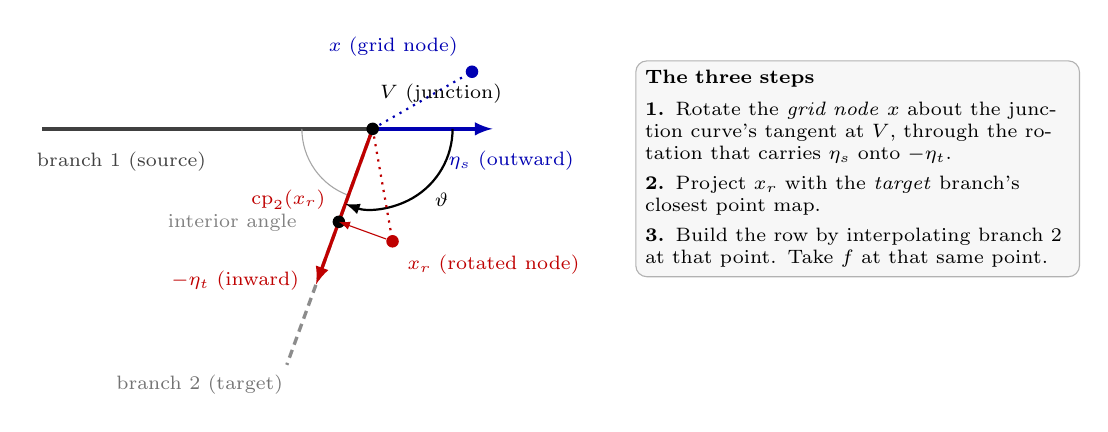
\begin{tikzpicture}[scale=1.45,>=latex,
    srcface/.style={very thick, black!75},
    tgtface/.style={very thick, black!45, densely dashed},
    node1/.style={circle, fill=blue!70!black, inner sep=1.6pt},
    node2/.style={circle, fill=red!75!black, inner sep=1.6pt},
    cp/.style={circle, fill=black, inner sep=1.6pt},
    lbl/.style={font=\scriptsize}]

  \coordinate (V) at (0,0);

  % ---- branch 1: the source face, along 180 degrees ----
  \draw[srcface] (V) -- (-2.90,0);
  \node[lbl, black!75, anchor=north] at (-2.20,-0.12)
      {branch 1 (source)};

  % ---- branch 2: the target face, along 250 degrees ----
  \draw[tgtface] (V) -- (-0.752,-2.067);
  \node[lbl, black!55, anchor=north east] at (-0.70,-2.07)
      {branch 2 (target)};

  % ---- the interior angle at the junction ----
  \draw[black!35] (-0.62,0) arc[start angle=180, end angle=250,
      radius=0.62];
  \node[lbl, black!50, anchor=north east] at (-0.58,-0.66)
      {interior angle};

  % ---- outward conormal of the source ----
  \draw[->, very thick, blue!70!black] (V) -- (1.05,0);
  \node[lbl, blue!70!black, anchor=north west] at (0.58,-0.11)
      {$\eta_s$ (outward)};

  % ---- inward direction of the target, along branch 2 ----
  \draw[->, very thick, red!75!black] (V) -- (-0.496,-1.363);
  \node[lbl, red!75!black, anchor=east] at (-0.56,-1.33)
      {$-\eta_t$ (inward)};

  % ---- the glue rotation ----
  \draw[->, thick, black] (0.70,0) arc[start angle=0,
      end angle=-110, radius=0.70];
  \node[lbl, anchor=west] at (0.46,-0.62) {$\vartheta$};

  % ---- the grid node, and its rotated image ----
  \node[node1] (X) at (0.87,0.50) {};
  \node[lbl, blue!70!black, anchor=south east] at (0.83,0.55)
      {$x$ (grid node)};
  \draw[blue!70!black, dotted, thick] (V) -- (X);

  \node[node2] (XR) at (0.174,-0.985) {};
  \node[lbl, red!75!black, anchor=north west] at (0.22,-1.02)
      {$x_r$ (rotated node)};
  \draw[red!75!black, dotted, thick] (V) -- (XR);

  % ---- the closest point of the rotated node on branch 2 ----
  \coordinate (CPT) at (-0.296,-0.814);
  \node[cp] at (CPT) {};
  \draw[->, red!75!black, thin] (XR) -- (CPT);
  \node[lbl, red!75!black, anchor=south east] at (-0.33,-0.79)
      {$\mathrm{cp}_2(x_r)$};

  \node[cp] at (V) {};
  \node[lbl, anchor=south west] at (-0.02,0.14) {$V$ (junction)};

  % ---- annotation box, clear of the drawing ----
  \node[draw=black!30, fill=black!3, rounded corners, align=left,
        lbl, text width=5.4cm, anchor=north west] at (2.30,0.60)
      {\textbf{The three steps}\\[1.2mm]
       \textbf{1.} Rotate the \emph{grid node} $x$ about the junction
          curve's tangent at $V$, through the rotation that carries
          $\eta_s$ onto $-\eta_t$.\\[1mm]
       \textbf{2.} Project $x_r$ with the \emph{target} branch's
          closest point map.\\[1mm]
       \textbf{3.} Build the row by interpolating branch 2 at that
          point. Take $f$ at that same point.};

\end{tikzpicture}
\caption{The angle rotation glue, drawn in the plane normal to the
  junction curve. Here $\eta_t$ is the target branch's \emph{outward}
  conormal, so branch 2 itself lies along $-\eta_t$. The rotation carries
  the source branch's outward direction $\eta_s$ onto $-\eta_t$. Leaving
  one branch means entering the other, so outward-onto-inward is the
  pairing a rigid continuation needs. The object that is rotated is the
  grid node $x$, not its closest point. This carries both the overhang
  past the junction and the normal offset across intact. On the ellipsoid
  this plane is a meridian half plane, and one angle serves the whole cut
  circle. On the tube the plane is the normal plane of a corner curve,
  and the angle varies along the curve, because the twist stops the two
  faces from being perpendicular.}
\label{fig:glue}
\end{figure}



\subsection{Which rows are rotated}

A row is rotated when its own closest point lies on the junction curve.

On the ellipsoid, \texttt{cpEllipseArc} returns the clamped end of the
meridian arc exactly. The test is therefore done on the meridian
coordinates $(\rho,z)$ of the closest point, with the reflection undone
first, to a tolerance of $10^4\,\varepsilon$. The poles are the other
ends of the two meridian arcs. They are not boundaries, because the
surface of revolution closes up there, and they are correctly not
matched.

On the tube, the closest point function returns a flag
$\mathrm{bdy}=\pm1$ when the closest point lies on the edge $s=\mp W$.
Every outer row with $\mathrm{bdy}\neq0$ is routed.

\subsection{The rotation axis}

The axis is the tangent to the junction curve at the row's own closest
point.

On the ellipsoid that tangent is the azimuthal direction
$e_\vartheta$. Two facts make this the honest lift of the planar
construction. First, the closest point $V$ of the node lies on a
\emph{circle}, so the offset of the node from $V$ has no $e_\vartheta$
component; the node lies in $V$'s own meridian half plane, and a rotation
about $e_\vartheta$ keeps it there. Second, the surface is one of
revolution, so the closest point of the rotated node on the other branch
lies in the same half plane. The whole construction is the planar one,
applied meridian by meridian, and the angle is the planar angle in the
$(\rho,z)$ coordinates of that half plane.

On the tube the axis is $\tau = F_\theta/|F_\theta|$ at the edge closest
point. Both strips share it. Both methods use the analytic $\tau$.

\subsection{The angle}

The glue carries the \emph{outward} direction of the source branch onto
the \emph{inward} direction of the target branch. Leaving the source
branch at the junction means entering the target branch, so
outward-onto-inward is the pairing a rigid continuation needs. On a
smooth join the two directions are opposite and the rotation is the
identity.

On the ellipsoid the two directions are the outward unit tangents of the
two meridian arcs at the cut. Reflecting branch~2 negates the $z$
component of its tangent, and that is what opens the crease. At
$s_0=0.6$, for example, the exact glue angle is $1.4282$~rad
($81.8^\circ$).

On the tube the two directions are the outward conormals,
\begin{equation}
  \eta_s = \operatorname{sign}(s)\,
  \mathrm{unit}\bigl(F_s - (F_s\!\cdot\!\tau)\tau\bigr),
\end{equation}
on the source strip, and $\eta_t$ likewise on the target strip at the
glued parameters. The glue carries $\eta_s$ onto $-\eta_t$. Because of
the twist this angle varies along the curve, so it is computed per row.

\subsection{The construction: Rodrigues, not \texttt{atan2}}

Nothing in this code stores a glue angle. The rotation is stored as a
$(\cos,\sin)$ pair, and the pair comes straight out of the two
directions. Rodrigues' formula about a unit axis $k$ is
\begin{equation}
  R = I + \sin\vartheta\,K + (1-\cos\vartheta)\,K^2 ,
  \qquad K = \mathrm{skew}(k) .
\end{equation}
In the plane the axis is $e_z$, $K^2=-I$, and the formula collapses to
$R = \cos\vartheta\,I + \sin\vartheta\,K = \begin{bmatrix} c & -s\\ s &
c\end{bmatrix}$ with
\begin{equation}
  c = u\cdot w , \qquad
  s = (u\times w)\cdot e_z = u_1w_2 - u_2w_1 ,
\end{equation}
followed by one division by $\mathrm{hypot}(c,s)$. In three dimensions
the same two quantities are $c = u\cdot w$ and
$s = \tau\cdot(u\times w)$. No angle is formed and no transcendental
function is evaluated.

The angle-first alternative reaches the same matrix through six library
transcendental calls, and $\cos$ and $\sin$ immediately undo what
\texttt{atan2} just did. Four consequences follow, and the planar
companion experiment measures all of them:
\begin{itemize}
  \item \textbf{Accuracy.} Against a rotation known to full precision,
        $\|R-R_{\mathrm{exact}}\|$ comes out two to seven times larger
        for the angle-first path at every angle sampled over a full turn.
        The worst case over that sweep is $1.2\times10^{-15}$ against
        $2.8\times10^{-16}$. Both are a few units in the last place, so
        this is a reason to prefer the construction, not a defect being
        repaired.
  \item \textbf{No branch cut.} A difference of two \texttt{atan2} values
        lands in $(-2\pi,2\pi]$ and must be wrapped back. The stored
        number is then discontinuous at $\pm\pi$, although the rotation
        it stands for is not. A $(\cos,\sin)$ pair has no such seam.
  \item \textbf{Exact inverses.} Swapping the two directions gives the
        other branch's glue at the same junction point. Under Rodrigues
        the cosine comes out bit for bit the same and the sine bit for
        bit negated, so the two branches' rotations are \emph{exact}
        transposes. The angle-first path satisfies that only to within
        rounding.
  \item \textbf{Reproducibility.} IEEE~754 pins down multiply, add,
        divide and \texttt{hypot}. It says nothing about \texttt{atan2},
        \texttt{sin} or \texttt{cos}. Dot products, cross products and
        \texttt{hypot} cannot differ between platforms; the angle-first
        matrix can.
\end{itemize}

\subsection{The estimated rotations}

The exact rotation uses analytic directions. It is the reference. Each
test also runs rotations built only from closest point differences,
because a real application has no analytic frame.

Write $\mathrm{cp}$ for the closest point of the node $x$ on its own
branch, and reflect the node through it:
\begin{align}
  \overline{\mathrm{cp}} &= \mathrm{cp}(2\,\mathrm{cp}-x), &
  \overline{\overline{\mathrm{cp}}} &= \mathrm{cp}(3\,\mathrm{cp}-2x) .
\end{align}
The two estimators are
\begin{align}
  d_k   &= \mathrm{cp} - \overline{\mathrm{cp}}
           &&\text{(first order)}, \\
  d_{k2} &= 1.5\,\mathrm{cp} - 2\,\overline{\mathrm{cp}}
            + 0.5\,\overline{\overline{\mathrm{cp}}}
           &&\text{(second order)} .
\end{align}
A plain difference of closest points returns nothing at these rows,
because the closest point \emph{is} the junction point. That is why the
node is reflected first.

\paragraph{Ellipsoid.} Each difference is resolved in its own node's
meridian frame $(e_\rho,e_z)$ \emph{before} averaging. By rotational
symmetry that is the frame the glue angle is measured in. Averaging the
raw vectors instead would cancel them around the circle. The
$e_\vartheta$ component is discarded; it is zero for the exact tangent
and only noise here. The script runs three variants per cut: $d_k$,
$d_{k2}$, and the exact rotation.

\paragraph{Tube.} Both conormals are estimated by $d_{k2}$, projected off
the exact $\tau$ and normalized. The source estimate reflects the
original routed grid node, $v = c-x$. A row is re-sampled with a
deterministic outward probe $x' = c + h\,\eta_s$ when any of these holds:
$|v|$ is tiny; the projected difference is short relative to $|v|$
($\alpha = |d_\perp|/|v| < 0.25$); a reflected closest point is itself on
an edge; the sample jumps to the opposite sheet; or the estimate points
inward. The target estimate always uses the outward probe
$c_t + h\,\eta_t$. An unusable probe raises an error; there is no
fallback to the exact conormal.

This makes the tube's $d_{k2}$ \emph{not} a fully geometry-free
estimator, and the script says so. The exact $\tau$ supplies the axis and
the projection plane. The exact conormals place the probes and check the
outward orientation. Both directions that set the angle are still closest
point differences.

\subsection{Applying the rotation}

We rotate the \emph{grid node}, never its closest point. That is what
makes the map a rigid continuation: both the tangential overhang past the
junction and the normal offset are carried across intact. Rotating the
closest point instead would only reparametrize the junction curve, and it
would lose the normal coordinate.

On the ellipsoid, the offset $x-V$ is resolved in the node's own meridian
frame into $(d_\rho, d_\vartheta, d_z)$. The planar rotation is applied
to $(d_\rho, d_z)$. The component $d_\vartheta$ is zero up to rounding,
and it is carried through anyway, so the formula does not quietly depend
on it vanishing. The result is mapped back to Cartesian coordinates.

On the tube, Rodrigues' formula is applied directly,
\begin{equation}
  x_r = c + (x-c)\cos\vartheta + \bigl(\tau\times(x-c)\bigr)\sin\vartheta
        + \tau\,\bigl(\tau\cdot(x-c)\bigr)(1-\cos\vartheta) ,
\end{equation}
again from the $(\cos,\sin)$ pair and not from an angle.

The rotated node is then projected with the \emph{target} branch's
closest point function. The interpolation stencil is built there.

\subsection{Measuring the rotation error}

The error of an estimated rotation is reported through the \emph{relative}
rotation $R_{\mathrm{exact}}^{\!\top} R$, whose angle lands in
$(-\pi,\pi]$ by construction:
\begin{equation}
  c_{\mathrm{rel}} = c\,c_{\mathrm{ref}} + s\,s_{\mathrm{ref}},
  \qquad
  s_{\mathrm{rel}} = s\,c_{\mathrm{ref}} - c\,s_{\mathrm{ref}} .
\end{equation}
There is nothing to re-wrap. The obvious alternative, a wrapped
difference of two angles, loses digits exactly where the comparison
matters, which is when both angles sit near $\pm\pi$.

\section{How we form the operator}

\subsection{Test 1: the vGMM operator}

The ellipsoid test uses the embedded method-of-lines operator of von
Glehn, M\"arz and Macdonald \cite{vGMM2013},
\begin{equation}
  M = EL - \gamma\,(I-E), \qquad \gamma = \frac{2d}{h^2},
  \label{eq:vgmm}
\end{equation}
and solves $(I-M)\,u = f$. Here $E$ is the degree-3 interpolation at the
closest points, square on the band, and $L$ is the second-order 7-point
Laplacian on the same band.

The glue needs no further handling, and that is the attraction of this
operator. $L$ is block diagonal, so
\begin{equation}
  (EL)_{k,o} = E_{k,o}\,L_o
\end{equation}
extends the \emph{other} branch's $Lu$ across the cut. The stabilization
row $u_i - (Eu)_i$ at a rotated node of branch $k$ is exactly the
statement that branch $k$'s value there agrees with branch $o$'s
interpolant at the rotated point. In assembly, a routed row's entry in
the diagonal block is zeroed, and its weights go into the off-diagonal
block.

$M$ is never assembled. In three dimensions $EL$ has some hundreds of
entries per row; $E$ and $L$ separately have 64 and 7. The operator is
applied as
\begin{equation}
  (I-M)\,v = (1+\gamma)\,v - E\bigl(Lv + \gamma v\bigr) ,
\end{equation}
under restarted GMRES with a Jacobi preconditioner built from
$\operatorname{diag}(EL)_i = \sum_j E_{ij}L_{ji}$. The tolerance is
$10^{-10}$, the restart is 40, and the cap is 400 restart cycles.

\paragraph{The forcing at a junction row.} A rotated row's unknown does
not stand for $u$ at that row's own closest point. That point is on the
cut circle. It stands for $u$ at the rotated target on the other branch,
which is up to $\mathrm{bw}\,h$ of arclength away. Its forcing is
therefore $f$ at the \emph{rotated target}.

This is the one place where the three-dimensional script deliberately
differs from its planar companion, and the reason is a counting argument.
Using $f$ at the row's own clamped closest point leaves a residual
$f(\text{target}) - f(V) = O(h)$ on every one of those rows. With $O(1)$
such rows in the plane that is invisible. With $O(1/h)$ of them around a
circle it is not.

That choice needs a caveat, because it is the convention the surface
analysis singles out as the dangerous one. Evaluating the forcing on the
opposite side without correcting a trace jump can leave the forcing
residual at $O(1)$ instead of $O(h)$, and that would promote its
contribution from $O(h^2)$ to $O(h)$. It is safe here only because
$[f]=0$: $u$ and $f$ are the same functions of $(\varphi,\vartheta)$ on
both branches, so the two one-sided traces agree and there is no jump to
correct. A forcing written per branch rather than per
$(\varphi,\vartheta)$ would break that, and would then need $f$ at the
source-side edge point or an explicit trace correction.

\paragraph{The baseline.} The same vGMM operator is also run on
\emph{one} band over the union of the two pieces. On the unflipped
surface that is the plain ellipsoid, and it measures the uncut rate. On
the flipped surface it is the closest point method applied to the crease
\emph{as if the crease were not there}. That is the other number worth
having.

\subsection{Test 2: the stabilized (diagonally split) ICPM operator}

The tube test uses the diagonally split operator. Let $L$ be the 7-point
Laplacian from the inner band rows to the outer band columns, and $R$ the
restriction from outer to inner. Split $L$ by its own diagonal,
\begin{equation}
  L_{\mathrm{diag}} = \textstyle\sum_j (R\odot L)_{ij}, \qquad
  L_{\mathrm{off}} = L - R\odot L ,
\end{equation}
and form
\begin{equation}
  M = \operatorname{diag}(L_{\mathrm{diag}})
      + L_{\mathrm{off}}\,E ,
  \label{eq:icpm}
\end{equation}
then solve $(I-M)\,u = R\,f_{\mathrm{out}}$.

The extension $E$ is split in two. $E_{\mathrm{self}}$ holds the
non-routed rows; the routed rows of the diagonal block are zeroed.
$E_{\mathrm{cross}}$ holds the routed rows, which interpolate the target
branch at the closest point of the rotated node.

The right-hand side is the source branch's $f$ at the outer rows. On a
routed row it is overwritten by the \emph{target} branch's $f$ at the
target closest point, for the same reason as above.

The solve is a sparse direct solve while the unknown count stays at or
below $25\,000$, and matrix-free restarted GMRES otherwise, with the
$(I-L_{\mathrm{diag}})$ diagonal preconditioner, tolerance $10^{-10}$,
restart 80 and 200 outer cycles. A GMRES failure is an error, not a
warning. The residual of the returned solution is recomputed and stored.

\subsection{What the scripts refuse to do}

Both tests are written so that a silently thinned band is impossible.
Each of the following raises an error rather than a warning:
\begin{itemize}
  \item an interpolation stencil of a closest point leaves the band;
  \item a cross-junction stencil leaves the \emph{other} band;
  \item a cross-junction stencil reads a row whose Laplacian stencil is
        incomplete;
  \item a row sum of the extension differs from one by more than
        $10^{-10}$;
  \item the band or routing closure does not converge in the allowed
        sweeps;
  \item the linear solve does not reach its residual target;
  \item a $d_{k2}$ probe is still unusable after the fallback probe.
\end{itemize}
The row sums and the linear residual are reported per level, so the
tables below can be read against them.

\section{How we measure the error}

The reported quantity is the surface $L_\infty$ error of the
\emph{interpolant}, not of the band values.

On the ellipsoid, each branch is sampled at the midpoints of a uniform
partition of its polar-angle interval, and around each parallel with a
count set by that parallel's own circumference. No sample falls exactly
on the cut circle or at a pole. A sample whose interpolation stencil is
not entirely inside the band is dropped and counted. The script also
records \emph{where} the worst point sits, as an arclength from the cut
circle in multiples of $h$. That is the test of whether the crease is
what hurts the solve.

On the tube, each strip is sampled on a uniform $(\theta,s)$ grid with
about two samples per $h$ in each direction, and \emph{both} edge curves
are included. The script also reports the trace discrepancy of the two
branches on each corner curve.

The ellipsoid test reports four further cross-branch measures at the
nodes the two bands have in common:
\begin{center}
\begin{tabular}{ll}
  \toprule
  measure & definition \\
  \midrule
  \texttt{gap}    & $\max|e_A - e_B|$ at the shared rotated nodes \\
  \texttt{vtx}    & $\max|u_A - u_B|$ on the cut circle \\
  \texttt{branch} & $\max(|e_A|, |e_B|)$ at the same nodes \\
  \texttt{allgap} & $\max|e_A - e_B|$ over the whole overlap \\
  \bottomrule
\end{tabular}
\end{center}
Each branch is compared against the value its \emph{own} unknown stands
for. At a crease the raw difference of the two unknowns is $O(h)$
whatever the scheme does, because the two unknowns stand for $u$ at
different points. What has to be compared is each branch's own error.


\section{Results: the flipped cap on an ellipsoid}
\label{sec:ellres}

\subsection{The geometry of one cut}

\begin{figure}[htbp]
\centering
\includegraphics[width=\textwidth]{flipped_vgmm_cut_z_0.39_error.png}
\caption{The cut at $z=0.39$, the one with the largest curvature
  mismatch of the four. Left: the meridian half plane. Branch~1 (blue) is
  the bowl. Branch~2 (red) is the cap, reflected down across the cut
  plane, so it runs \emph{inside} the bowl and the two meet at the star
  in a crease of $81.8^\circ$. The two arrows are the outward tangents
  the glue rotation is built from. Right: the surface $\Linf$ error
  against $h$. The heavy black line is the uncut solve with the crease
  ignored; it is flat. The three glued variants lie on top of one
  another, and their sawtooth is the grid-alignment scatter, not a
  failure of the solve.}
\label{fig:cut039}
\end{figure}

\subsection{The glue is what makes the solve converge}

The clearest result of this test is the gap between the baseline and the
glued solves. Table~\ref{tab:cut039} gives the cut at $z=0.39$ in full.

\begin{table}[htbp]
\centering
\caption{Surface $\Linf$ error of $u$, flipped ellipsoid, cut at
  $z=0.39$ ($\varphi_c = 0.9273$, $\kappa_m = 1.2986$,
  $\kappa_p = 0.8187$, glue angle $1.4282$~rad $= 81.8^\circ$,
  $\dk = 3.0703$). The rate under each error is the level-to-level
  ratio. Only the fitted slope is a rate; see
  Section~\ref{sec:scatter}.}
\label{tab:cut039}
\small
\begin{tabular}{@{}r rr rr rr rr@{}}
\toprule
 & \multicolumn{2}{c}{uncut, crease ignored}
 & \multicolumn{2}{c}{rotation from $d_k$}
 & \multicolumn{2}{c}{rotation from $d_{k2}$}
 & \multicolumn{2}{c}{exact $R$} \\
\cmidrule(lr){2-3}\cmidrule(lr){4-5}\cmidrule(lr){6-7}\cmidrule(lr){8-9}
$h$ & error & rate & error & rate & error & rate & error & rate \\
\midrule
0.0650  & 4.071e-01 & --    & 2.101e-02 & --    & 6.599e-02 & --    & 2.244e-02 & --    \\
0.0533  & 3.467e-01 & 0.81  & 1.149e-02 & 3.04  & 1.697e-02 & 6.84  & 1.145e-02 & 3.39  \\
0.0437  & 3.566e-01 & $-0.14$ & 3.057e-03 & 6.67  & 5.507e-03 & 5.67  & 3.261e-03 & 6.33  \\
0.0358  & 2.970e-01 & 0.92  & 1.074e-02 & $-6.33$ & 1.149e-02 & $-3.70$ & 1.089e-02 & $-6.07$ \\
0.0294  & 5.391e-01 & $-3.00$ & 3.403e-03 & 5.79  & 3.046e-03 & 6.69  & 3.356e-03 & 5.93  \\
0.0241  & 2.836e-01 & 3.24  & 6.445e-03 & $-3.22$ & 6.414e-03 & $-3.75$ & 6.436e-03 & $-3.28$ \\
\midrule
\multicolumn{1}{@{}l}{fitted}
        & \multicolumn{2}{c}{\textbf{0.10}}
        & \multicolumn{2}{c}{1.20}
        & \multicolumn{2}{c}{2.31}
        & \multicolumn{2}{c}{\textbf{1.26}} \\
\bottomrule
\end{tabular}
\end{table}

Three things are worth reading off it.

\paragraph{The baseline does not converge.} The uncut vGMM solve, which
applies the closest point method to the creased surface as if the crease
were not there, has a fitted slope of $0.10$. Its error stays between
$0.28$ and $0.54$ at every grid spacing. It is $O(1)$. That is the
expected behaviour: at the crease the closest point map of the union
surface is not single valued, so the extension has no consistent
footpoint, and refining the grid does not repair it.

\paragraph{The glue converges, at about first order.} The glued solves
drop the error by about 1.7 orders of magnitude, to
$6.4\times10^{-3}$ at the finest level, and the fitted slope of the
exact rotation is $1.26$. This is well short of the second-order rate a
smooth closest point solve would give, and it is what
Equation~\eqref{eq:bound3} predicts: with $\dk$ (and hence $D$) a
definite nonzero number, the term $h\,D$ sits at first order and
dominates $h^2$.

\paragraph{The three rotations are the same solve.} At the three finest
levels the three variants agree to within 7 per cent, and at the finest
level to within 0.5 per cent: $6.445$, $6.414$ and
$6.436 \times 10^{-3}$. The differences between their fitted slopes
($1.20$, $2.31$, $1.26$) are therefore \emph{not} a difference between
the schemes. They are an artifact of where the scatter falls on the
coarse levels, where $d_{k2}$ starts three times worse than the other
two. The glue rotation does not have to be exact for this solve: it has
to be good enough, and both estimators are.

\subsection{Why a level-to-level rate is meaningless here}
\label{sec:scatter}

The per-level rates in Table~\ref{tab:cut039} run from $-6.33$ to
$+6.84$. The error is not monotone: it falls to $3.3\times10^{-3}$ at
$h=0.0437$, rises to $1.1\times10^{-2}$ at $h=0.0358$, falls again, and
rises again at the finest level.

This is the behaviour the script's own header predicts, and it is not
noise in the solver. The residual of the solve is below $10^{-10}$ at
every level and the extension row sums are correct to $10^{-15}$. The
size of the surface error is set by the net \emph{signed} junction
residual summed around the cut circle. That sum is a near cancellation
between the two branches: each contributes a systematic total of one
sign and the other the opposite sign. What survives depends on where the
cut circle happens to fall between grid planes, which changes with $h$ in
a way that has nothing to do with accuracy.

The position of the worst point confirms this. The script reports its
distance from the cut circle in multiples of $h$:

\begin{center}
\small
\begin{tabular}{@{}rrrrrr@{}}
\toprule
$h$ & 0.0650 & 0.0533 & 0.0437 & 0.0358 & 0.0294 \\
\midrule
worst point, in units of $h$ from the crease
    & 0.9 & 0.3 & 10.5 & 0.5 & 0.6 \\
\bottomrule
\end{tabular}
\end{center}

At five of the six levels the worst point sits within one grid cell of
the crease, which says the crease is what limits the solve. At
$h=0.0437$, the one level where the error dips, it has moved ten cells
away: at that grid alignment the junction residual cancelled, and what
was left was the ordinary interior error.

In the plane the same cancellation exists. There the junction is two
points instead of a circle, the sums run over $O(1)$ rows instead of
$O(1/h)$ rows, and the scatter never surfaces.

\paragraph{A caveat on the fit.} The script's default is ten grid
spacings, and the reason is precisely to average over this scatter. The
runs in this report use \emph{six}, because the finer levels of the
default list cost more than the time available. The fitted slopes here
are therefore less well determined than the script intends. They should
be read as "first order, not second", not as three-digit numbers.

\subsection{The cross-branch measures}

The four cross-branch measures behave better than the surface error,
because they do not depend on the signed cancellation around the circle.
For the cut at $z=0.39$ the fitted slopes are:

\begin{center}
\small
\begin{tabular}{@{}llrrr@{}}
\toprule
measure & what it is & $d_k$ & $d_{k2}$ & exact $R$ \\
\midrule
\texttt{gap}    & $\max|e_A-e_B|$ at the shared rotated nodes & 2.90 & 4.68 & 1.97 \\
\texttt{vtx}    & $\max|u_A-u_B|$ on the cut circle           & 1.96 & 3.26 & 1.76 \\
\texttt{branch} & $\max(|e_A|,|e_B|)$ at the same nodes       & 1.35 & 3.49 & 1.21 \\
\texttt{allgap} & $\max|e_A-e_B|$ over the whole overlap      & 2.90 & 4.68 & 1.98 \\
\bottomrule
\end{tabular}
\end{center}

The two branches agree with each other at close to second order
(\texttt{gap} and \texttt{allgap}, $1.97$ and $1.98$ for the exact
rotation), and they agree on the cut circle itself at $1.76$. The
\texttt{branch} measure, which is each branch's own error at those nodes,
tracks the surface error at $1.21$. So the glue is \emph{consistent}
across the junction to better than the order at which either branch is
\emph{accurate}. The limit is not the transmission; it is the crease.

\subsection{The estimated rotations}

The fitted rates of the angle error
$|\vartheta - \vartheta_{\mathrm{exact}}|$ at this cut are
\begin{center}
$d_k$: $2.13$, \qquad $d_{k2}$: $3.60$.
\end{center}
Both are better than the nominal order of the underlying difference. The
reason is the averaging: each closest point difference is resolved in its
own node's meridian frame and then averaged over the whole cut circle, so
the leading error term, which is odd around the circle, cancels.

In absolute terms, however, $d_k$ is the \emph{better} estimator over the
whole range tested:

\begin{center}
\small
\begin{tabular}{@{}rrrrrrr@{}}
\toprule
$h$ & 0.0650 & 0.0533 & 0.0437 & 0.0358 & 0.0294 & 0.0241 \\
\midrule
$d_k$    & 1.10e-02 & 4.43e-03 & 2.98e-03 & 2.61e-03 & 1.45e-03 & 1.15e-03 \\
$d_{k2}$ & 1.62e-01 & 8.42e-02 & 2.88e-02 & 1.75e-02 & 7.26e-03 & 5.27e-03 \\
\bottomrule
\end{tabular}
\end{center}

$d_{k2}$ starts two orders of magnitude worse and is still $4.6$ times
worse at the finest level. Its steeper slope means it would overtake
eventually, but it has not done so on any grid in this study. Neither
difference reaches the solution: at the finest three levels both
estimators give the same surface error as the exact rotation.

\subsection{All four cuts, against the curvature mismatch}
\label{sec:dkappa}

% Four-cut summary, drawn from the logged numbers.
% The script's own summary PNG covers only the three cuts of one process,
% because cut 1 was run separately; this figure carries all four.
\begin{figure}[htbp]
\centering
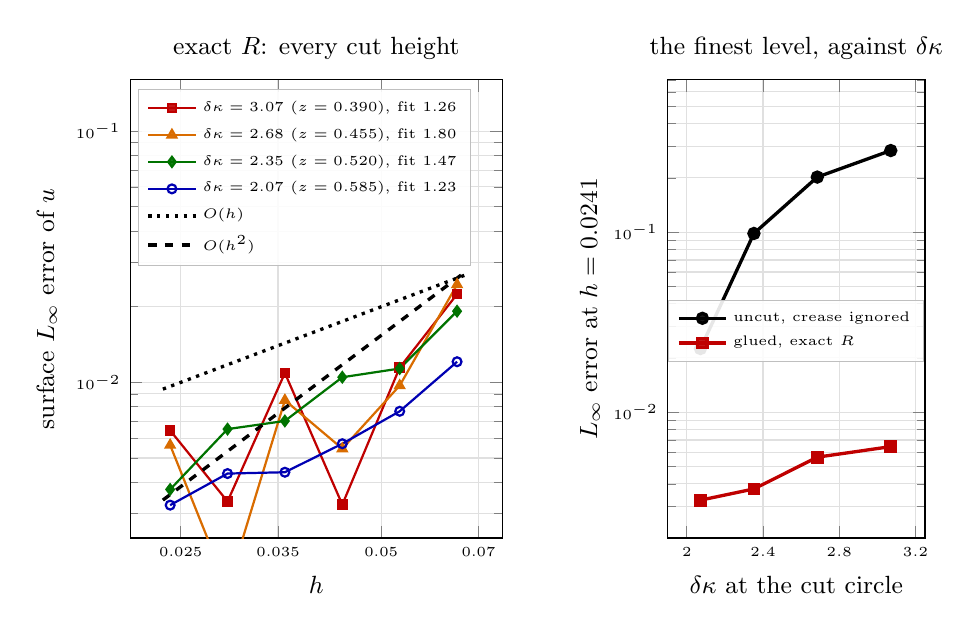
\begin{tikzpicture}

\begin{loglogaxis}[
  name=left,
  width=0.52\textwidth, height=7.4cm,
  xlabel={$h$}, ylabel={surface $\Linf$ error of $u$},
  title={\small exact $R$: every cut height},
  title style={yshift=-2pt},
  legend style={font=\tiny, at={(0.02,0.98)}, anchor=north west,
                draw=black!25, fill=white, fill opacity=0.9,
                text opacity=1, legend columns=1, row sep=0.5pt},
  legend cell align=left,
  xmin=0.021, xmax=0.076, ymin=2.4e-3, ymax=0.16,
  grid=both, grid style={black!12},
  tick label style={font=\tiny}, label style={font=\small},
  xtick={0.025,0.035,0.05,0.07},
  xticklabels={0.025,0.035,0.05,0.07},
]

\addplot[red!75!black, thick, mark=square*, mark size=1.5]
  coordinates {
    (0.065,2.244e-2) (0.053300,1.145e-2) (0.043706,3.261e-3)
    (0.035839,1.089e-2) (0.029388,3.356e-3) (0.024098,6.436e-3)};
\addlegendentry{$\dk=3.07$ ($z=0.390$), fit 1.26}

\addplot[orange!85!black, thick, mark=triangle*, mark size=1.8]
  coordinates {
    (0.065,2.451e-2) (0.053300,9.706e-3) (0.043706,5.444e-3)
    (0.035839,8.485e-3) (0.029388,1.516e-3) (0.024098,5.624e-3)};
\addlegendentry{$\dk=2.68$ ($z=0.455$), fit 1.80}

\addplot[green!45!black, thick, mark=diamond*, mark size=1.8]
  coordinates {
    (0.065,1.920e-2) (0.053300,1.135e-2) (0.043706,1.048e-2)
    (0.035839,7.020e-3) (0.029388,6.515e-3) (0.024098,3.747e-3)};
\addlegendentry{$\dk=2.35$ ($z=0.520$), fit 1.47}

\addplot[blue!70!black, thick, mark=o, mark size=1.6]
  coordinates {
    (0.065,1.208e-2) (0.053300,7.672e-3) (0.043706,5.697e-3)
    (0.035839,4.387e-3) (0.029388,4.334e-3) (0.024098,3.245e-3)};
\addlegendentry{$\dk=2.07$ ($z=0.585$), fit 1.23}

\addplot[black, dotted, very thick, domain=0.0235:0.067, samples=2]
  {2.6e-2*x/0.065};
\addlegendentry{$O(h)$}

\addplot[black, dashed, very thick, domain=0.0235:0.067, samples=2]
  {2.6e-2*(x/0.065)^2};
\addlegendentry{$O(h^2)$}

\end{loglogaxis}

\begin{semilogyaxis}[
  name=right, at={(left.east)}, anchor=west, xshift=2.1cm,
  width=0.40\textwidth, height=7.4cm,
  xlabel={$\dk$ at the cut circle},
  ylabel={$\Linf$ error at $h=0.0241$},
  ylabel style={yshift=-2pt},
  title={\small the finest level, against $\dk$},
  title style={yshift=-2pt},
  legend style={font=\tiny, at={(0.5,0.52)}, anchor=north,
                draw=black!25, fill=white, fill opacity=0.9,
                text opacity=1},
  legend cell align=left,
  xmin=1.9, xmax=3.25, ymin=2e-3, ymax=0.7,
  grid=both, grid style={black!12},
  tick label style={font=\tiny}, label style={font=\small},
  xtick={2.0,2.4,2.8,3.2},
]

\addplot[black, very thick, mark=*, mark size=1.8]
  coordinates {(2.0720,2.255e-2) (2.3525,9.824e-2)
               (2.6849,2.020e-1) (3.0703,2.836e-1)};
\addlegendentry{uncut, crease ignored}

\addplot[red!75!black, very thick, mark=square*, mark size=1.7]
  coordinates {(2.0720,3.245e-3) (2.3525,3.747e-3)
               (2.6849,5.624e-3) (3.0703,6.436e-3)};
\addlegendentry{glued, exact $R$}

\end{semilogyaxis}

\end{tikzpicture}
\caption{All four cut heights. Left: the surface $\Linf$ error of the
  glued solve with the exact rotation, against $h$. The uncut baseline is
  left out of this panel, because it is two orders of magnitude higher;
  it appears in Figure~\ref{fig:cut039} and in the right panel here. All
  four glued curves sit between the $O(h)$ and $O(h^2)$ guides, and all
  four zigzag. Right: the error at the finest level, against the
  curvature mismatch $\dk$. Both the baseline and the glued solve order
  monotonically by $\dk$, although the \emph{fitted slopes} do not ---
  see the text below.}
\label{fig:cutsummary}
\end{figure}


The four cut heights span crease angles from $34.9^\circ$ to
$81.8^\circ$, and with them a range of curvature mismatch.
Table~\ref{tab:fourcuts} collects them.

\begin{table}[htbp]
\centering
\caption{All four cuts of the flipped ellipsoid. $\dk$ falls as the cut
  moves from the equator towards the pole. Each entry is the fitted
  slope over six levels, with the error at the finest level
  ($h=0.0241$) beside it.}
\label{tab:fourcuts}
\footnotesize
\setlength{\tabcolsep}{4pt}
\begin{tabular}{@{}rrcrr rr rr rr rr@{}}
\toprule
 & & & &
 & \multicolumn{2}{c}{uncut, crease ignored}
 & \multicolumn{2}{c}{$d_k$}
 & \multicolumn{2}{c}{$d_{k2}$}
 & \multicolumn{2}{c}{exact $R$} \\
\cmidrule(lr){6-7}\cmidrule(lr){8-9}\cmidrule(lr){10-11}\cmidrule(lr){12-13}
$z$ & $\varphi_c$ & crease & $\kappa_m$ & $\dk$
 & rate & error & rate & error & rate & error & rate & error \\
\midrule
0.390 & 0.9273 & $81.8^\circ$ & 1.2986 & 3.0703
 & 0.10 & 2.84e-01 & 1.20 & 6.45e-03 & 2.31 & 6.41e-03 & 1.26 & 6.44e-03 \\
0.455 & 0.7954 & $67.1^\circ$ & 1.0970 & 2.6849
 & 0.59 & 2.02e-01 & 1.78 & 5.60e-03 & 2.20 & 5.80e-03 & 1.80 & 5.62e-03 \\
0.520 & 0.6435 & $52.0^\circ$ & 0.9220 & 2.3525
 & 0.33 & 9.82e-02 & 1.47 & 3.74e-03 & 1.89 & 3.70e-03 & 1.47 & 3.75e-03 \\
0.585 & 0.4510 & $34.9^\circ$ & 0.7738 & 2.0720
 & 1.00 & 2.25e-02 & 1.22 & 3.26e-03 & 1.22 & 3.28e-03 & 1.23 & 3.24e-03 \\
\bottomrule
\end{tabular}
\end{table}

\paragraph{The error level orders by $\dk$. The fitted rate does not.}
This is the main qualification on this test. At the finest level the
error of the glued solve falls monotonically as $\dk$ falls:
\begin{equation*}
  6.44,\quad 5.62,\quad 3.75,\quad 3.25 \;\;(\times 10^{-3})
  \qquad\text{for}\qquad
  \dk = 3.07,\; 2.68,\; 2.35,\; 2.07 .
\end{equation*}
The uncut baseline does the same, and far more strongly: from
$2.84\times10^{-1}$ down to $2.25\times10^{-2}$, a factor of 12.

The fitted slopes, by contrast, are $1.26$, $1.80$, $1.47$ and $1.23$.
They do not order by $\dk$, and they do not order by anything else
either. Six levels are not enough to separate a trend in the rate from
the grid-alignment scatter of Section~\ref{sec:scatter}. The defensible
statement from this study is therefore:

\begin{quote}
  Every cut converges at a fitted rate between $1.2$ and $1.8$. None
  reaches second order. The size of the error at a fixed grid spacing
  grows with $\dk$, as Equation~\eqref{eq:bound3} says it should ---
  through the constant in $C\,h\,D$, not through the exponent.
\end{quote}

That is how a bound behaves when its junction term is first order with a
$\dk$-dependent constant. Changing $\dk$ moves the curve up and down. It
would change the \emph{rate} only if $\dk$ reached zero. The unflipped
cut, where $\dk$ vanishes identically, is the test of that. It is the
\texttt{flipped = false} branch of the script, and it is not run here.

\paragraph{Where the error sits.} The script reports the distance of the
worst point from the cut circle, in units of $h$. At the two sharpest
cuts that distance is within one cell at nearly every level. At the
mildest cut, $z=0.585$, it is $11.5$, $14.1$ and $16.6$ cells at the
three coarsest levels, and it moves to the crease only at the three
finest. At a mild crease the junction is not the worst thing in the
solve until the grid is fine enough for the interior error to fall below
it.

\paragraph{The estimated rotations, across all cuts.} At every cut the
three variants agree at the finest level to within 1 per cent. The
fitted rates of the angle error are $2.13$, $2.30$, $2.36$ and $1.98$
for $d_k$, and $3.60$, $3.25$, $3.76$ and $2.93$ for $d_{k2}$. Both
estimators beat the nominal order of their underlying difference at
every cut, and neither difference reaches the solution.



\section{Results: the half-twisted rectangular tube}
\label{sec:tuberes}

\begin{figure}[htbp]
\centering
\includegraphics[width=\textwidth]{half_twisted_rectangular_tube_geometry.png}
\caption{The half-twisted rectangular tube and its two face-pair strips.
  Left: the complete surface, which is a closed orientable torus. Middle:
  the wide strip, $p=(s,b)$ with $s\in[-a,a]$. Right: the narrow strip,
  $p=(a,s)$ with $s\in[-b,b]$. Each strip covers its face pair once over
  $\theta\in[0,4\pi)$, and each is an annulus, not a M\"obius strip. The
  red and the blue curve are the two closed corner curves where the
  strips meet. The cross-section sides are straight, but the faces they
  sweep are not planar.}
\label{fig:tubegeom}
\end{figure}

\subsection{The bands and the routed rows}

\begin{figure}[htbp]
\centering
\includegraphics[width=0.92\textwidth]{half_twisted_rectangular_tube_narrow_band.png}
\caption{The two narrow bands at $h=1/22$, and the nodes the glue
  rotates. Blue dots are the outer band of branch~A, orange rings the
  outer band of branch~B, and magenta the rows that are routed across a
  corner curve. A node that lies in both bands carries both markers,
  because it carries two independent unknowns.}
\label{fig:tubeband}
\end{figure}

The routed rows are not a thin shell. Table~\ref{tab:tubesize} gives the
counts. At every level about one unknown in five is a row whose value is
supplied by the glue rather than by its own branch. That is the reason
the junction term in Equation~\eqref{eq:bound} is not a local
perturbation on this surface: there are two closed junction curves, and
every one of their neighbourhoods is routed.

\begin{table}[htbp]
\centering
\caption{Problem size and solver behaviour, half-twisted rectangular
  tube. Routed rows are summed over both branches and both corner
  curves. The row-sum error is $\max_i |\sum_j E_{ij} - 1|$.}
\label{tab:tubesize}
\small
\begin{tabular}{@{}rrrrrrr@{}}
\toprule
$h$ & unknowns A & unknowns B & routed rows & GMRES iter
    & rel.\ residual & row-sum error \\
\midrule
0.05000 &  32\,393 & 17\,391 & 21\,029 &  722 & 9.7e-11 & 1.3e-15 \\
0.04000 &  49\,040 & 25\,556 & 26\,686 &  840 & 9.9e-11 & 1.6e-15 \\
0.03333 &  68\,599 & 34\,963 & 31\,930 & 1203 & 9.9e-11 & 1.6e-15 \\
0.02778 &  96\,784 & 48\,138 & 37\,808 & 1544 & 9.9e-11 & 1.6e-15 \\
0.02273 & 141\,729 & 69\,344 & 46\,307 & 2276 & 1.0e-10 & 1.6e-15 \\
\bottomrule
\end{tabular}
\end{table}

\subsection{Convergence of the $\Linf$ error}

\begin{figure}[htbp]
\centering
\includegraphics[width=\textwidth]{half_twisted_rectangular_tube_rotation_convergence.png}
\caption{Left: the surface $\Linf$ error of both rotations, with $O(h)$
  and $O(h^2)$ guides. The two curves lie on top of one another. The
  error starts between the guides and bends towards $O(h)$ as $h$ falls.
  Right: the worst $d_{k2}$ rotation angle error, against an $O(h^2)$
  guide. It falls faster than second order.}
\label{fig:tubeconv}
\end{figure}

\begin{table}[htbp]
\centering
\caption{Surface $\Linf$ error of $u$, combined over both strips,
  half-twisted rectangular tube with $R=1$, $a=0.45$, $b=0.20$. Rates
  use the actual $h$ ratios.}
\label{tab:tubeconv}
\small
\begin{tabular}{@{}r rr rr r@{}}
\toprule
 & \multicolumn{2}{c}{exact rotation}
 & \multicolumn{2}{c}{$d_{k2}$ rotation}
 & $d_{k2}$ worst \\
\cmidrule(lr){2-3}\cmidrule(lr){4-5}
$h$ & error & rate & error & rate & angle error (rad) \\
\midrule
1/20 & 1.4041e-01 & --   & 1.4018e-01 & --   & 1.3967e+00 \\
1/25 & 8.5293e-02 & 2.23 & 8.5201e-02 & 2.23 & 6.7693e-01 \\
1/30 & 6.3814e-02 & 1.59 & 6.3876e-02 & 1.58 & 2.6388e-01 \\
1/36 & 5.4570e-02 & 0.86 & 5.4621e-02 & 0.86 & 1.3056e-01 \\
1/44 & 4.4203e-02 & 1.05 & 4.4186e-02 & 1.06 & 6.2282e-02 \\
\midrule
\multicolumn{1}{@{}l}{fitted}
     & \multicolumn{2}{c}{\textbf{1.429}}
     & \multicolumn{2}{c}{\textbf{1.426}}
     & 4.04 \\
\bottomrule
\end{tabular}
\end{table}

\paragraph{The fitted rate is 1.43, and it is not an asymptotic order.}
Table~\ref{tab:tubeconv} gives a least-squares slope of $1.429$ for the
exact rotation. That number alone is misleading, because the
level-to-level rates fall steadily:
\begin{equation*}
  2.23, \quad 1.59, \quad 0.86, \quad 1.05 .
\end{equation*}
The solve starts close to second order on the coarsest pair and settles
near first order on the finest pairs. Figure~\ref{fig:tubeconv} shows the
same thing: the error curve starts below the $O(h^2)$ guide and bends
towards the $O(h)$ guide. The fitted $1.429$ is an average over a range
in which the rate is still changing, not the order the scheme will hold
at smaller $h$. The honest statement is that the observed behaviour is
consistent with a first-order junction term taking over from a
second-order interior term, which is what Equation~\eqref{eq:bound}
predicts when $D$ and $J_2$ do not vanish.

Unlike the ellipsoid, this surface has no grid-alignment scatter: the
error is monotone in $h$ at every level. The two junction curves are not
plane circles, and the glue angle varies along them, so the signed
junction residual does not add up to a near cancellation that depends on
grid position.

\paragraph{Cross-check against the recorded run.} The notes in
\texttt{angle\_rotation\_glue.md} record a run at
$h\in\{1/25, 1/30, 1/40\}$. The three levels this study shares with it
reproduce it to every printed digit: $8.5293\mathrm{e}{-2}$ and
$6.3814\mathrm{e}{-2}$ for the exact rotation, $8.5201\mathrm{e}{-2}$ and
$6.3876\mathrm{e}{-2}$ for $d_{k2}$, and the level rate $1.59$ for the
pair $1/25 \to 1/30$.

\subsection{The estimated rotation costs nothing here}

The two rotations are indistinguishable in the solution. The largest
relative difference over all five levels is $0.16$ per cent, at the
coarsest level, and at the finest level the $d_{k2}$ solve is marginally
the \emph{better} of the two ($4.4186$ against
$4.4203 \times 10^{-2}$). That is not a real advantage; it is the size
of the difference.

This holds although the $d_{k2}$ rotation is a poor estimate on the
coarse grids. Its worst angle error is $1.40$~rad at $h=1/20$, which is
$80^\circ$ on the worst row. The error falls at a fitted rate of $4.04$,
with level rates $3.25$, $5.17$, $3.86$ and $3.69$, reaching
$6.2\times10^{-2}$~rad at the finest level.

\paragraph{How many rows need the fallback probe.} The $d_{k2}$ source
estimate is re-sampled from the deterministic outward probe
$c + h\,\eta_s$ whenever the reflected ray is unusable. The counts are
substantial and they grow with refinement:

\begin{center}
\small
\begin{tabular}{@{}rrrr@{}}
\toprule
$h$ & probed rows, branch A & probed rows, branch B & sign reversals \\
\midrule
1/20 & 2972 & 1789 & 7 \\
1/25 & 3100 & 2248 & 0 \\
1/30 & 3000 & 2609 & 0 \\
1/36 & 3360 & 3107 & 0 \\
1/44 & 3973 & 3854 & 0 \\
\bottomrule
\end{tabular}
\end{center}

So roughly one routed row in six falls back to the probe. The probe is
placed with the \emph{analytic} conormal, which is why this variant is
not a geometry-free estimator, as the script states. The seven sign
reversals at the coarsest level are rows where the long reflected sample
misjudged which side of the edge it was on.

\subsection{The traces agree at nearly second order}

The two branches agree with each other on the corner curves far better
than either agrees with the exact solution:

\begin{center}
\small
\begin{tabular}{@{}rrr@{}}
\toprule
$h$ & $\max|u_A-u_B|$, upper curve & $\max|u_A-u_B|$, lower curve \\
\midrule
1/20 & 2.879e-02 & 2.765e-02 \\
1/25 & 1.610e-02 & 2.123e-02 \\
1/30 & 1.219e-02 & 1.288e-02 \\
1/36 & 7.763e-03 & 1.144e-02 \\
1/44 & 6.412e-03 & 7.186e-03 \\
\midrule
\multicolumn{1}{@{}l}{fitted} & \textbf{1.93} & \textbf{1.71} \\
\bottomrule
\end{tabular}
\end{center}

The trace discrepancy converges at $1.93$ and $1.71$, against $1.43$ for
the surface error itself, and this is the same pattern the ellipsoid
shows. The glue transmits consistently across the junction at close to
second order. What limits the solve is not the transmission.


\section{What the two tests say together}
\label{sec:together}

\subsection{The bound the two tests are read against}

The surface analysis \cite{MMC2026b} gives, for the glued solve,
\begin{equation}
  \bigl\| Q_h u_h - u \bigr\|_\infty
  \;\le\; C\Bigl\{ h^{q} + h^{p-1} + h\,(D + J_2) + h^2
          + \varepsilon_R + h\,\rho_{f,h} \Bigr\} ,
  \label{eq:bound}
\end{equation}
conditional on a discrete stability assumption. With $q=2$ and $p=3$,
and with a source-consistent forcing convention, this reads
\begin{equation}
  \bigl\| Q_h u_h - u \bigr\|_\infty
  \;\le\; C\bigl\{ h^2 + h\,(D + J_2) + \varepsilon_R \bigr\} .
  \label{eq:bound2}
\end{equation}
Three constants in \eqref{eq:bound2} decide what the tables can show.

\paragraph{$D$, the extrinsic junction defect.} $D$ is the supremum over
the junction curve of $|b_2^\perp - b_1^\perp|$, the mismatch of only the
\emph{mixed} and \emph{transverse} parts $(b_{sr}, b_{rr})$ of the second
fundamental form in the matched edge frame. On the flipped ellipsoid the
meridian and the parallel are the principal directions of both branches,
so $b_{sr}=0$ on both and
\begin{equation}
  D = 2\kappa_m .
\end{equation}
The along-edge curvature $\kappa_p$ drops out of $D$, because the
transmission conditions already match $U_{ss}$.

\paragraph{$\dk$, the quantity the tables report.} The ellipsoid script
reports instead
\begin{equation}
  \dk = \bigl\| \mathrm{II}_1 - R\,\mathrm{II}_2 R^{\!\top} \bigr\|_F ,
\end{equation}
the full matched-frame mismatch, which \cite{MMC2026b} calls a valid but
less sharp replacement for $D$. On this family $\dk$ runs 18 to 34 per
cent above $D$, and it is monotone in the same direction, so ranking the
cuts by either gives the same order.

The script builds $\dk$ rather than assuming it. Both branches are pieces
of the same ellipsoid, met at the same $\varphi_c$, so they share
\begin{equation}
  \kappa_m = \frac{ac}{G^{3/2}}, \qquad
  \kappa_p = \frac{c}{a\sqrt{G}}, \qquad
  G(\varphi) = a^2\cos^2\!\varphi + c^2\sin^2\!\varphi ,
\end{equation}
and the mismatch collapses to $|n_1 - Rn_2|\sqrt{\kappa_m^2+\kappa_p^2}$
with $n$ the inward unit normals. On the \emph{unflipped} cut, $R$ is the
identity and $n_2=n_1$, so $\dk$ vanishes identically and the glued solve
should recover the second-order rate of the uncut one. On the
\emph{flipped} cut, $R$ carries $n_2$ to $-n_1$, so $|n_1-Rn_2|=2$ and
\begin{equation}
  \dk = 2\sqrt{\kappa_m^2 + \kappa_p^2}
  \qquad\text{(flipped)}
\end{equation}
at every cut height. It varies only through where on the meridian the cut
falls.

\paragraph{$J_2$, the intrinsic junction defect.} $J_2$ is
$[U_{rr}] = (k_2-k_1)U_r - [f]$, with $k_i$ the geodesic curvature of the
junction curve inside branch $i$. On the flipped ellipsoid it vanishes,
and \emph{both} of its terms vanish separately. The two branches are
mirror images across the cut plane, so $k_2=k_1$. And $u$ and $f$ are the
same functions of $(\varphi,\vartheta)$ on both branches, so $[f]=0$.

That is a different route to $J_2=0$ than the two-sphere example of
\cite{MMC2026b}, where the two terms are individually nonzero and cancel.
On the flipped ellipsoid the whole junction defect is therefore
\emph{extrinsic}, and the bound reads
\begin{equation}
  \bigl\| Q_h u_h - u \bigr\|_\infty
  \;\le\; C\bigl\{ h^2 + h\,D + \varepsilon_R \bigr\} .
  \label{eq:bound3}
\end{equation}

\paragraph{$\varepsilon_R$, the rotation error.} This is the term the
estimated rotations pay and the exact rotation does not. It is the only
term that separates the three variants of the ellipsoid test, and the
only term that separates \texttt{exact} from \texttt{dk2} on the tube.

\paragraph{$\rho_{f,h}$, the forcing residual.} This is why both scripts
take $f$ at the \emph{rotated target} on a routed row. Evaluating the
forcing on the opposite side without correcting a trace jump can leave
$\rho_{f,h}=O(1)$ instead of $O(h)$. That would promote $h\rho_{f,h}$
from $O(h^2)$ to $O(h)$ and put it on a level with the junction term
itself. It is safe in both tests only because $[f]=0$ by construction.


\subsection{The two surfaces are different tests of the same thing}

The two surfaces differ in nearly every way that could matter, which is
what makes the agreement between them useful.

\begin{center}
\small
\begin{tabular}{@{}lll@{}}
\toprule
 & flipped ellipsoid & half-twisted tube \\
\midrule
junction      & one plane circle & two closed non-planar curves \\
glue angle    & one angle for the whole circle
              & varies along each curve \\
operator      & vGMM, $M = EL - \gamma(I-E)$
              & diagonally split ICPM \\
solve         & matrix-free GMRES
              & direct, then matrix-free GMRES \\
$J_2$         & zero, both terms separately
              & nonzero in general \\
estimators    & $d_k$ and $d_{k2}$, fully geometry-free
              & $d_{k2}$, with analytic axis and probes \\
scatter in $h$ & large & none \\
fitted rate   & 1.23 to 1.80 & 1.43 \\
\bottomrule
\end{tabular}
\end{center}

They agree on the three things that matter. First, the rate is between
first and second order and nearer to first. Second, the glue rotation may
be estimated rather than computed, at no cost in the solution. Third, the
junction transmission converges faster than the solution does.

\subsection{Why the ellipsoid scatters and the tube does not}

This is the sharpest contrast in the study, and it is worth stating
plainly, because it changes how each table must be read.

On the ellipsoid the junction is a circle in a plane, and the glue
rotation is one angle for every point of it. Each branch therefore
contributes a junction residual of one sign at every azimuth, and the two
contributions very nearly cancel. What survives is set by where the
circle falls between grid planes. That changes with $h$ in a way that has
nothing to do with accuracy, so neighbouring levels differ by a factor of
several.

On the tube neither corner curve is planar, and the twist makes the glue
angle vary along both. The residuals do not line up in azimuth, nothing
near-cancels, and the error is monotone in $h$ at every level.

The practical consequence: a convergence study on a surface of revolution
cut by a plane needs many more levels than one on a generic surface. The
ellipsoid script's choice of ten grid spacings is not conservatism.

\subsection{What would settle the open question}

The one experiment that would separate the two candidate explanations is
already in the script and was not run here: the \emph{unflipped} cut.

On the unflipped surface the two pieces join smoothly, the exact glue
rotation is the identity, and $\dk$ vanishes identically. The bound then
reads $C\{h^2 + \varepsilon_R\}$, and the glued solve should recover the
second-order rate of the uncut one. If it does, then the order lost on
the flipped surface is the \emph{crease}, and the glue itself is
second-order accurate. If it does not, then the glue construction costs
an order by itself, independently of the geometry it is applied to.

Nothing in this report distinguishes those two possibilities, because
every cut studied here has $\dk$ between $2.07$ and $3.07$ and none has
$\dk = 0$.

Two smaller follow-ups are worth the same note:

\begin{itemize}
  \item \textbf{More levels on the ellipsoid.} The script's own default
        of ten would make the four fitted rates comparable with one
        another. At six levels they are not.
  \item \textbf{Finer levels on the tube.} Its level rates were still
        falling at $h=1/44$. One or two more levels would show whether
        they settle at first order or continue down.
\end{itemize}

\subsection{A note on the construction, separate from the results}

The $(\cos,\sin)$ construction of the rotation is a correctness and
reproducibility choice, not an accuracy one. The measured difference
against the \texttt{atan2} path is a few units in the last place, and the
planar companion experiment shows it does not reach the computed
solution. What it does buy is exact: the two branches' rotations at a
junction come out as bit-for-bit transposes, there is no branch cut at
$\pm\pi$ for a stored angle to fall across, and every operation is one
that IEEE~754 pins down. Those properties hold regardless of the rates in
this report.


\section{How to reproduce}
\label{sec:repro}

All of the numbers in this report come from the two scripts named below.
Run them from their own directory. No argument is needed for the first
one.

\begin{verbatim}
cd cp_matrices/examples_2026/3D_surface

matlab -batch "example_ellipsoid_flipped_cap_branch_consistency_vgmm"

matlab -batch "example_half_twisted_rectangular_tube_rotation_convergence(1./[20 25 30 36 44])"
\end{verbatim}

\subsection{Two changes were needed to produce these runs}

\paragraph{A bug stops the ellipsoid script after its first cut.} In
\texttt{example\_ellipsoid\_flipped\_cap\_branch\_consistency\_vgmm.m},
the local function \texttt{error\_surface\_figure} is declared with
twenty parameters, ending \texttt{geoname, dkappa}. Its body then uses
\texttt{thetaex(1)}:

\begin{verbatim}
                     dkappa, thetaex(1)*180/pi, dx)}, 'FontSize', 9);
\end{verbatim}

\texttt{thetaex} is never passed to it. A local function in a script file
does not share the script's workspace, so this raises
\texttt{Unrecognized function or variable 'thetaex'}. The default
\texttt{z\_3d = 0.390} is not empty, so the figure is always requested,
and the script always aborts after the first cut height. It therefore
never reaches cuts two, three and four, nor the summary tables, nor the
summary figure.

The fix is to pass the variable through. Add \texttt{thetaex} to the end
of the function's parameter list, and to the end of its call. The call
site already has \texttt{thetaex} in scope: it is computed once per cut
height, just above.

\paragraph{The grid spacings were reduced.} The default list is
$h_k = 0.065\times 0.82^{\,k}$ for $k=0,\dots,9$. At four cut heights and
four solves per level, with the band size growing like $h^{-2}$, that is
a run of roughly a day. The runs here use $k=0,\dots,5$, which is the
same list truncated. Nothing else in the script was changed. The
consequences for the fitted rates are discussed in
Section~\ref{sec:scatter}.

\paragraph{Cut one was run separately.} Because the abort above was found
after cut one had completed, the first cut height comes from one process
and the other three from another. The two processes used identical
settings apart from \texttt{s0\_list} and \texttt{z\_3d}. The script's
own end-of-run summary figure therefore shows only three cuts;
Figure~\ref{fig:cutsummary} in this report is drawn from the logged
numbers of both processes and shows all four.

\paragraph{Supporting files.} The two scripts share the rotation
helpers and the geometry routines:

\begin{center}
\begin{tabular}{@{}ll@{}}
  \toprule
  file & what it does \\
  \midrule
  \texttt{rotations/rot2d\_from\_to.m}
    & the plane rotation carrying one direction onto another, by
      Rodrigues' formula \\
  \texttt{rotations/glue\_rot2d.m}
    & the same, with the junction convention: outward onto inward \\
  \texttt{rotations/rotate\_about2d.m}
    & applies a $(\cos,\sin)$ pair about a junction point \\
  \texttt{rotations/rot2d\_err.m}
    & the angle and matrix error of a rotation, through the relative
      rotation \\
  \texttt{3D\_surface/angle3D.m}
    & the same construction in three dimensions \\
  \texttt{surfaces/cpEllipseArc.m}
    & closest point of an arc of an ellipse, with an edge flag \\
  \texttt{surfaces/cpHalfTwistedRectTube.m}
    & closest point of one strip of the tube, with an edge flag \\
  \texttt{surfaces/halfTwistedRectTubeFrame.m}
    & the tube parametrization and its analytic derivatives \\
  \texttt{3D\_surface/halfTwistedRectTubeMMS.m}
    & the manufactured solution of the tube \\
  \texttt{3D\_surface/halfTwistedRectTubeBands.m}
    & the grid, the two bands, and the routing targets, per level \\
  \bottomrule
\end{tabular}
\end{center}

\paragraph{Figures.} Each script writes its own PNG files into
\texttt{examples\_2026/figs/}. The tube script also writes a MAT file
with the full \texttt{results} structure. The two plot-only scripts
\texttt{example\_half\_twisted\_rectangular\_tube\_geometry.m} and
\texttt{example\_half\_twisted\_rectangular\_tube\_narrow\_band.m}
produce Figures~\ref{fig:tubegeom} and~\ref{fig:tubeband}. They solve
nothing.

\paragraph{Theory notes.} \texttt{examples\_2026/angle\_rotation\_glue.md}
carries the derivation. Section~3 covers the glue rotation step by step,
and Section~10 covers the tube.


\begin{thebibliography}{9}

\bibitem{vGMM2013}
I.~von Glehn, T.~M\"arz and C.~B.~Macdonald.
\newblock An embedded method-of-lines approach to solving partial
  differential equations on surfaces.
\newblock 2013.

\bibitem{RuuthMerriman2008}
S.~J.~Ruuth and B.~Merriman.
\newblock A simple embedding method for solving partial differential
  equations on surfaces.
\newblock \emph{J.~Comput.~Phys.}, 2008.
\newblock (the bandwidth formula)

\bibitem{MMC2026}
T.~M\"arz, C.~B.~Macdonald and Y.~Chen.
\newblock Consistency and stability of closest point iterations.
\newblock Draft.

\bibitem{MMC2026b}
T.~M\"arz, C.~B.~Macdonald and Y.~Chen.
\newblock Closest point rotation across a shared surface edge: local
  proofs and conditional convergence in $\mathbb{R}^3$.
\newblock Draft, \texttt{output/pdf/cpm\_surface\_edge\_analysis.pdf}.
\newblock Theorem~6.4 is the bound quoted in this report;
  Assumption~6.3 is the discrete stability it is conditional on;
  Proposition~7.1 is what the uncut baseline measures.

\end{thebibliography}

\end{document}
